


	\subsubsection{Factor Analysis}
	The proposed procedure has been tested on the SPECT database (see Section~\ref{sec:vdlnhmpao} for a detailed description). Input parameters $K$ and $N$ have been varied in a large range of values to evaluate the effect of these parameters on the final results. Best results for AD detection have been obtained for $N=3000$ and $K=14$. Here we obtain an accuracy up to $0.937$, sensitivity up to $0.951$ and specificity up to $0.927$, along with a Positive and Negative Likelihood of $13.079$ and $0.053$ respectively.
	\begin{figure*}% Son los del experimento distances
		\centering
		\subfloat[PPMI database]{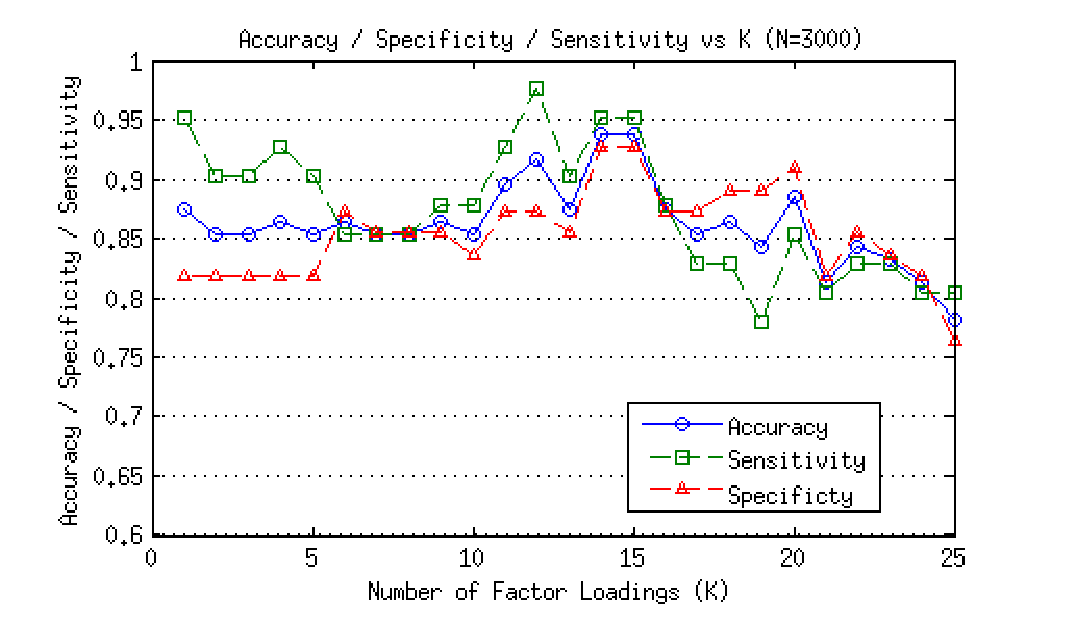
\includegraphics[width=0.45\textwidth]{gfx/ch4/accuracyMWW-K-N3}\label{fig:accMWW-K-N3}}
		\subfloat[VDLN database]{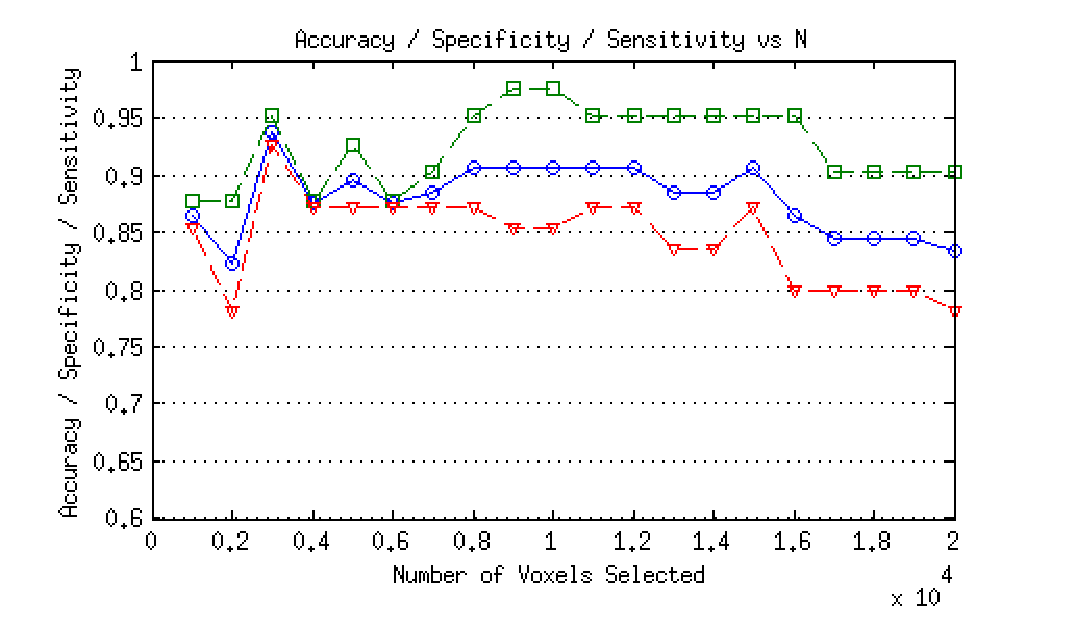
\includegraphics[width=0.45\textwidth]{gfx/ch4/accuracyMWW-N-K14}\label{fig:accuracyMWW-N-K14}}
		\subfloat[VDLV database]{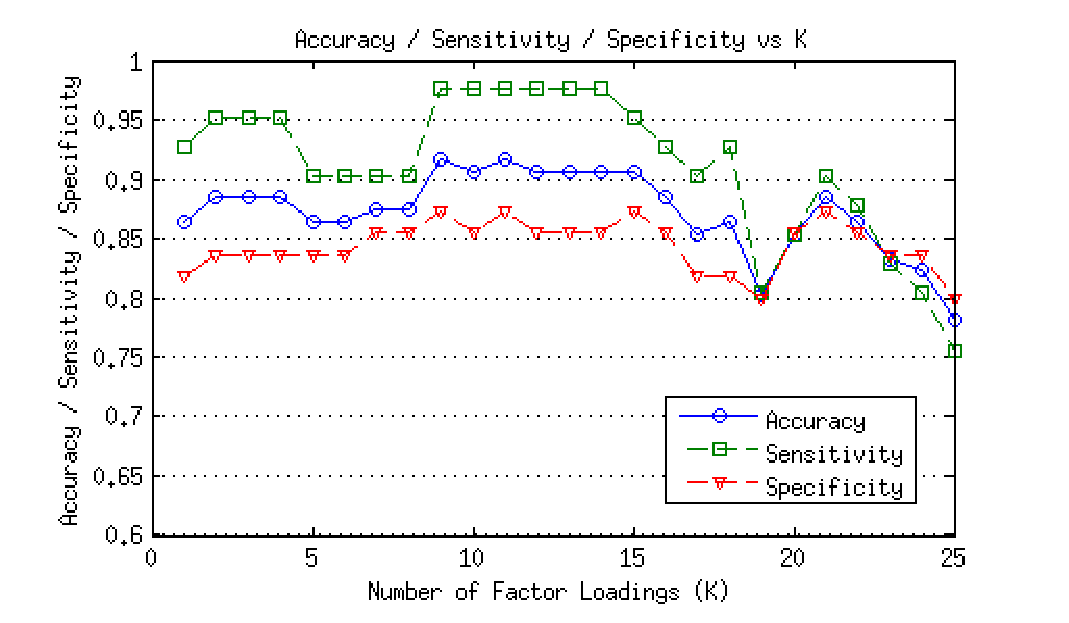
\includegraphics[width=0.45\textwidth]{gfx/ch4/accuracyMWW-K-N10}\label{fig:accuracyMWW-K-N10}}
		\subfloat[VDLV database]{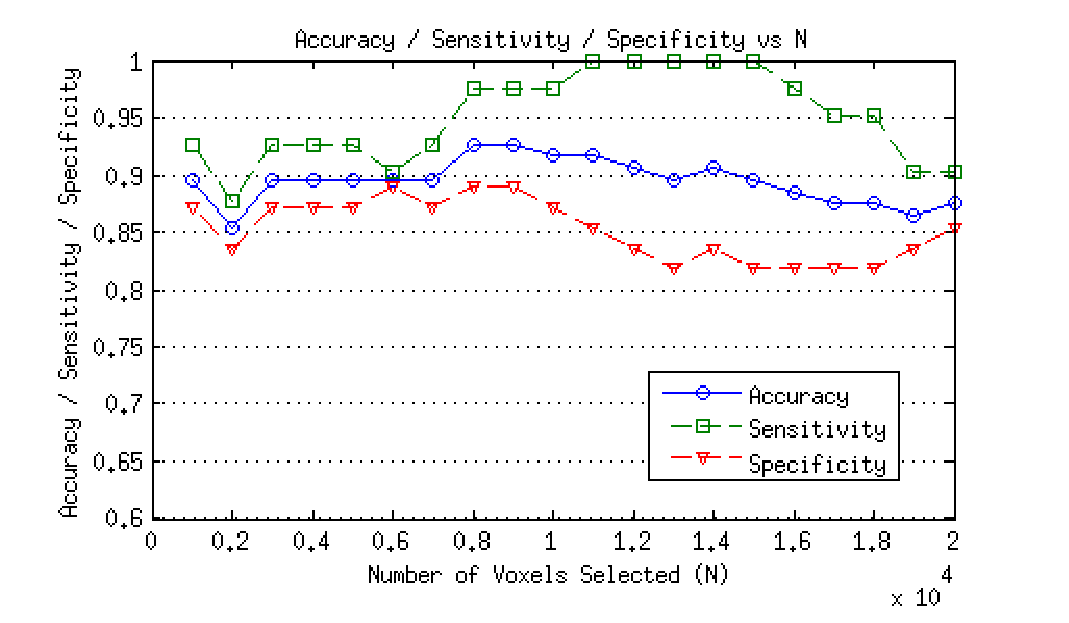
\includegraphics[width=0.45\textwidth]{gfx/ch4/accuracyMWW-N-K11}\label{fig:accuracyMWW-N-K11}}
		
		\caption{Values of accuracy, sensitivity and specificity computed for SPECT database in function of number of voxels selected (N) and number of features extracted (K), fixing \protect\subref{fig:accMWW-K-N3} $N=3000$, \protect\subref{fig:accuracyMWW-N-K14} $K=14$, \protect\subref{fig:accuracyMWW-K-N10} $N=10000$ and \protect\subref{fig:accuracyMWW-N-K11} $K=11$.}
		\label{fig:spectResults}
	\end{figure*}
	
	Fig. \ref{fig:spectResults} depicts values of accuracy, sensitivity and specificity in function of $N$ and $K$. In \ref{fig:spectResults}.a and \ref{fig:spectResults}.b, values of accuracy may fall from 0.94 to 0.85 within two steps in $K$ and increases from 0.83 to 0.94 in only one step of $N$. The same occurs when looking at the rest or parameters. These values are clearly peak values, and may indicate that they depend on the database used for testing.
	
	However, in \ref{fig:spectResults}.c and \ref{fig:spectResults}.d, we can see that there are a wide range of values where accuracy exceeds 0.9, for $N \in (5000, 13000)$ and $K \in (9, 15)$. In this area of interest, a small variation of the input parameters leads to a small variation in the results obtained, demonstrating that it is a robust method. This area coincides also with a similar one for the ADNI database, as we will see in Section \ref{discussion}, which may indicate that the area is also database-independent.
	
	%\subsubsection{ADNI-PET database}\label{adni}
	The variety of samples coming from different origins makes the ADNI database (see Sec. \ref{adniDB}) appealing for testing algorithms aiming at detecting AD. A larger number of patients are included in the database, that offers a wide variety of brain function patterns that range from NORMAL to AD.
	
	Due to the large number of images that this database contains, the system shows less variation between different input patterns, but there are still some peak values that does not correspond to the area of interest mentioned in previous section. The best results for the ADNI database gives us an accuracy up to 0.929, sensitivity of 0.911, specificity of 0.947, and positive and negative Likelihood of $17.307$ and $0.094$ in $N=6000$ and $K=23$.
	
	\begin{figure*}[ht]
		\centering
		\begin{tabular}{cc}
			a)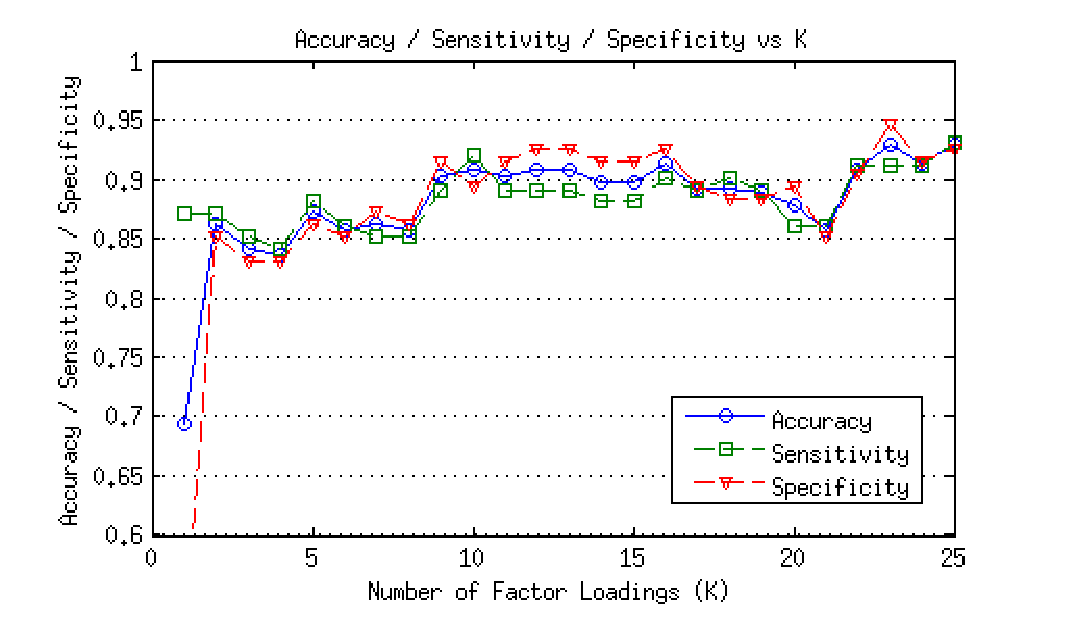
\includegraphics[width=0.45\textwidth]{gfx/ch4/accuracyMWW-K-N6-ADNI} & b)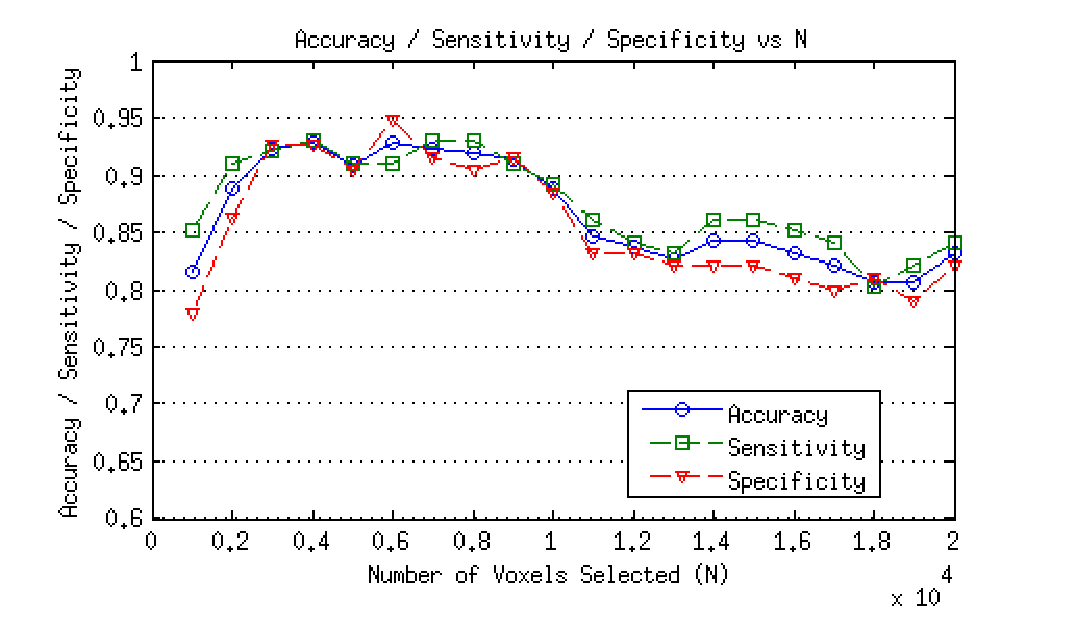
\includegraphics[width=0.45\textwidth]{gfx/ch4/accuracyMWW-N-K23-ADNI}\\
			c)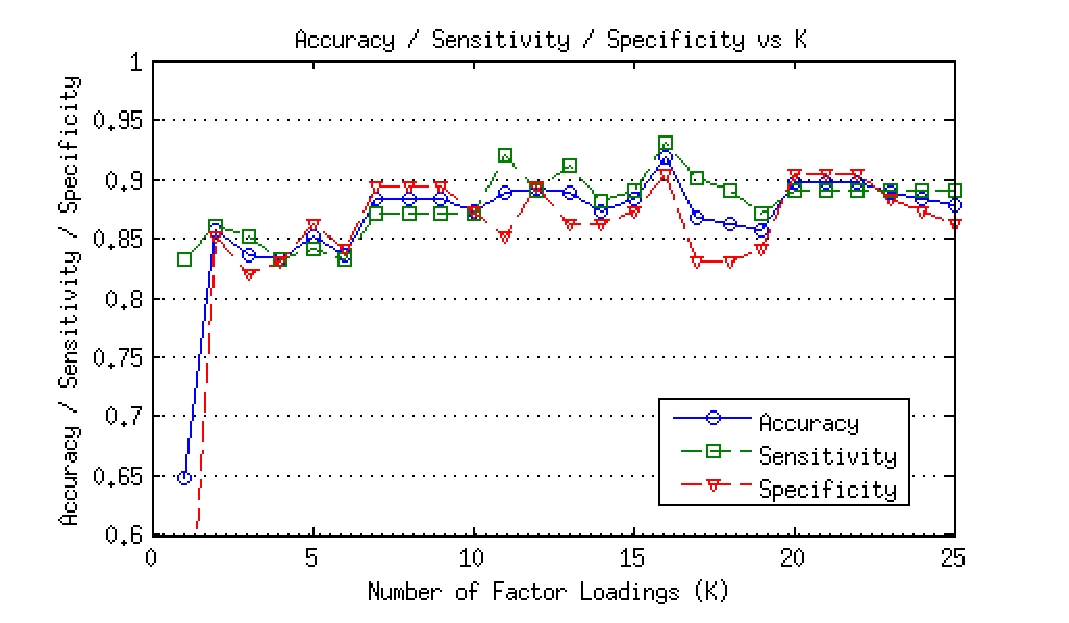
\includegraphics[width=0.45\textwidth]{gfx/ch4/accuracyMWW-K-N10-ADNI} & d)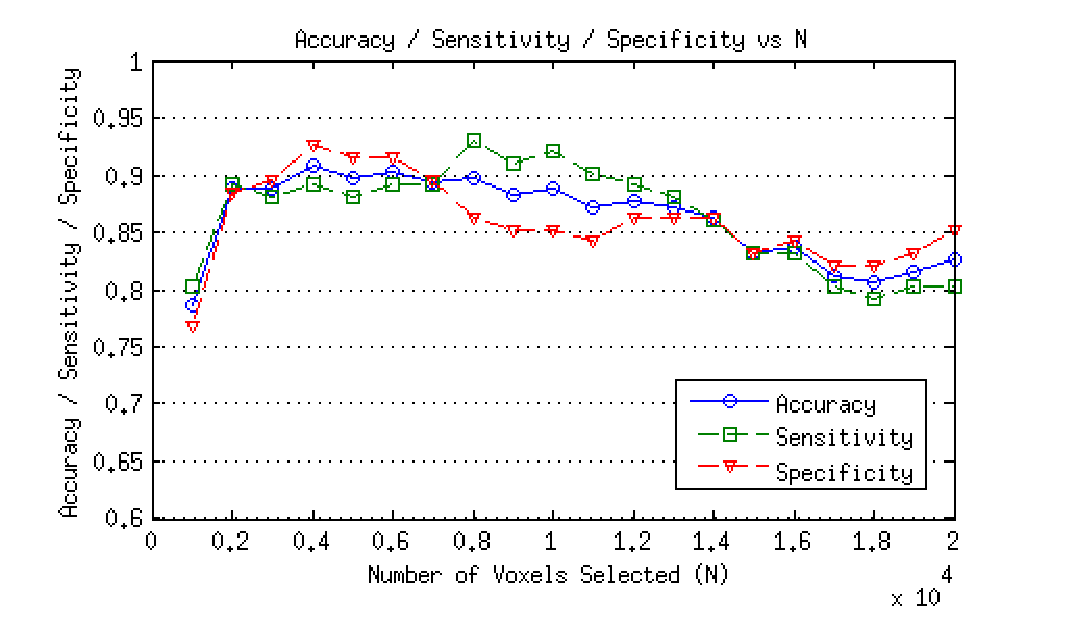
\includegraphics[width=0.45\textwidth]{gfx/ch4/accuracyMWW-N-K11-ADNI}\\
		\end{tabular}
		\caption{Values of accuracy, sensitivity and specificity computed for ADNI database in function of number of voxels selected (N) and number of features extracted (K), fixing \textit{a)} $N=6000$, \textit{b)} $K=23$, \textit{c)} $N=10000$ and \textit{d)} $K=11$. }
		\label{fig:petResults}
	\end{figure*}
	
	Figure \ref{fig:petResults} shows values of the accuracy, sensitivity and specificity as a function of $K$ and $N$. As in the previous case, this highest accuracy may decrease significantly when varying $K$ (from 0.93 to 0.86 when decreasing from $K=23$ to $K=21$, as seen in \ref{fig:petResults}.a), although \ref{fig:petResults}.b shows that accuracy is less likely to vary when increasing or decreasing $N$. However, there is a remarkable fall in the value of the accuracy when $N$ is incremented from $9000$ to $11000$. The same happens to sensitivity and specificity values. PL values vary from 17.3 to 5.8 in two steps of $K$ and from 10.8 to 5.1 in the case of decreasing $N$ from 9000 to 11000. The same occurs to NL values.
	
	Within the area of interest defined in previous section, Figs. \ref{fig:petResults}.c and \ref{fig:petResults}.d shows that the behaviour is repeated, although accuracy values slightly decrease. The range of $N$ is extended, yet sensitivity decreases after several values. Variations in $K$ have a little more influence on the final result, but the system retains its good sensitivity and accuracy values.
	
	\subsubsection{Independent Component Analysis}
	In this section the combination of different selection criteria and classifiers along with the feature extraction based on Independent Component Analysis will be analysed. The following classifiers have been tested in order to compare the performance results: Linear and Quadratic Normal Multivariate Classifier (MV Linear and MV Quadratic) \cite{Krzanowski88}, Naive Bayes Classifiers with either linear and quadratic discriminant function (introduced above), a classifier that makes use of the Mahalanobis distance to compute the class membership \cite{McLachlan1992} and SVM classifiers\cite{Vapnik1998} with linear, quadratic, polynomial and Radial Basis Function kernels (SVM Linear, Quadratic, Polynomial and RBF). 
	
	To obtain a general view of the results that these different combinations yield, values of accuracy obtained for each combination of classifier, selection criteria and database are shown on Table \ref{tab:icaMaxAcc}. Peak values of accuracy could have been displayed in this table, but we have opted for averaging the 10\% higher accuracy results obtained using each system, in order to provide us with an idea of both performance and stability, and thus, help us in the task of choosing the best system. 
	
	\begin{table*}[ht]
		\centering
		\begin{tabular}{ccccccc}
			& \multicolumn{3}{c}{SPECT} & \multicolumn{3}{c}{ADNI} \\
			\hline \hline
			Classifier & $t$-Test & Entropy & Wilcoxon & $t$-Test & Entropy & Wilcoxon \\
			\hline \hline
			MV Linear & 0.902 & 0.896 & 0.902 & 0.887 & \textbf{0.894} & \textbf{0.893} \\
			Bayes Linear & 0.923 & 0.916 & 0.896 & 0.835 & 0.878 & \textbf{0.893} \\
			MV Quadratic & 0.935 & \textbf{0.942} & 0.924 & 0.877 & 0.888 & 0.889 \\
			Bayes Quadratic & 0.934 & \textbf{0.951} & 0.924 & 0.816 & 0.884 & 0.873 \\
			Mahalanobis & 0.895 & 0.892 & 0.896 & 0.857 & 0.842 & 0.851 \\
			SVM Linear & 0.904 & 0.886 & 0.902 & 0.882 & \textbf{0.893} & \textbf{0.891} \\
			SVM Polinomial & 0.888 & 0.899 & 0.885 & 0.852 & 0.865 & 0.865 \\
			SVM Quadratic & 0.898 & \textbf{0.942} & 0.901 & 0.865 & 0.874 & 0.862 \\
			SVM RBF & 0.928 & \textbf{0.953} & 0.916 & 0.866 & 0.879 & 0.859 \\
			\hline
			\hline
		\end{tabular}
		\caption{Average values computed for the first 10\% highest accuracy evaluations performed using leave-one-out cross-validation for different combinations of classifiers, selection criteria and databases. }
		\label{tab:icaMaxAcc}
	\end{table*}
	
	Regarding the SPECT database, best accuracy results are obtained by using Relative Entropy selection criteria, with values up to $96.9\%$. With this database, the best classifiers are the Multivariate and Bayesian Quadratic, and SVM-RBF. On the other hand, the ADNI database achieves its best accuracy results when using linear classifiers, along with the wilcoxon and Relative Entropy selection criteria. Since the variance of parameters estimated using leave-one-out method might be high, a $k$-Fold estimation with $k=10$ may be the best option when choosing an statistical procedure \cite{Kohavi1995a}. Table \ref{tab:icaMaxAccK} shows the average values obtained by $k$-Fold using also the 10\% higher accuracy scores for each combination.
	
	\begin{table*}[ht]
		\centering
		\begin{tabular}{ccccccc}
			& \multicolumn{3}{c}{SPECT} & \multicolumn{3}{c}{ADNI} \\
			\hline \hline
			Classifier & $t$-Test & Entropy & Wilcoxon & $t$-Test & Entropy & Wilcoxon \\
			\hline 
			MV Linear & 0.901 & 0.899 & 0.905 & 0.889 & \textbf{0.894} & 0.889 \\
			Bayes Linear & 0.924 & 0.915 & 0.894 & 0.834 & 0.878 & \textbf{0.893} \\
			MV Quadratic & 0.934 & \textbf{0.941} & 0.924 & 0.872 & 0.886 & 0.888 \\
			Bayes Quadratic & 0.933 & \textbf{0.950} & 0.924 & 0.817 & 0.886 & 0.873 \\
			Mahalanobis & 0.899 & 0.890 & 0.900 & 0.857 & 0.841 & 0.852 \\
			SVM Linear & 0.896 & 0.890 & 0.898 & 0.883 & \textbf{0.892} & 0.883 \\
			SVM Polinomial & 0.888 & 0.900 & 0.882 & 0.849 & 0.864 & 0.866 \\
			SVM Quadratic & 0.902 & 0.938 & 0.900 & 0.863 & 0.872 & 0.856 \\
			SVM RBF & 0.929 & \textbf{0.951} & 0.917 & 0.863 & 0.878 & 0.857 \\
			\hline
			\hline
		\end{tabular}
		\caption{Average values computed for the first 10\% highest accuracy evaluations performed using $k$-Fold cross-validation for different combinations of classifiers, selection criteria and databases. }
		\label{tab:icaMaxAccK}
	\end{table*}
	
	The combinations that we had highlighted previously are confirmed by examining the above Table, as the best results are obtained with the Relative Entropy criteria in both databases, and non-linear classifiers (for SPECT database) and linear classifiers (for ADNI database). Highest accuracy, sensitivity and specificity values for SPECT database are obtained with the Relative Entropy selection criteria and a Bayesian Quadratic classifier, with values of $0.958$, $0.951$ and $0.964$ respectively. In the case of ADNI database, highest accuracy, sensitivity and specificity values are obtained with Relative Entropy and a SVM Linear classifier, yielding to values of $0.883$, $0.861$ and $0.905$ respectively. 
	
	
	With all these measures, we consider the combination of Entropy selection criteria and Bayesian Quadratic classifier the most robust system for the SPECT database. For the ADNI database, multivariate Lineal and SVM Linear classifier obtain similar results. Since the highest accuracy value is achieved with SVM Linear, we finally decide on this. 
	
	\subsubsection{VDLN-HMPAO}
	Figure \ref{fig:icaSPECTTodos} depicts the accuracy, sensitivity and specificity results by means of the number of selected voxels as input vector to the feature extraction step and by means of the number of components extracted by ICA. In these figures, the measures are presented along with the accuracy, sensitivity and specificity values obtained for the baseline method based on a Relative Entropy voxel selection. 
	
	\begin{figure*}[bth]
		\myfloatalign
		\subfloat[Accuracy, Sensitivity and Specificity in function of $N$]
		{\label{fig:baseSPvdln}%
			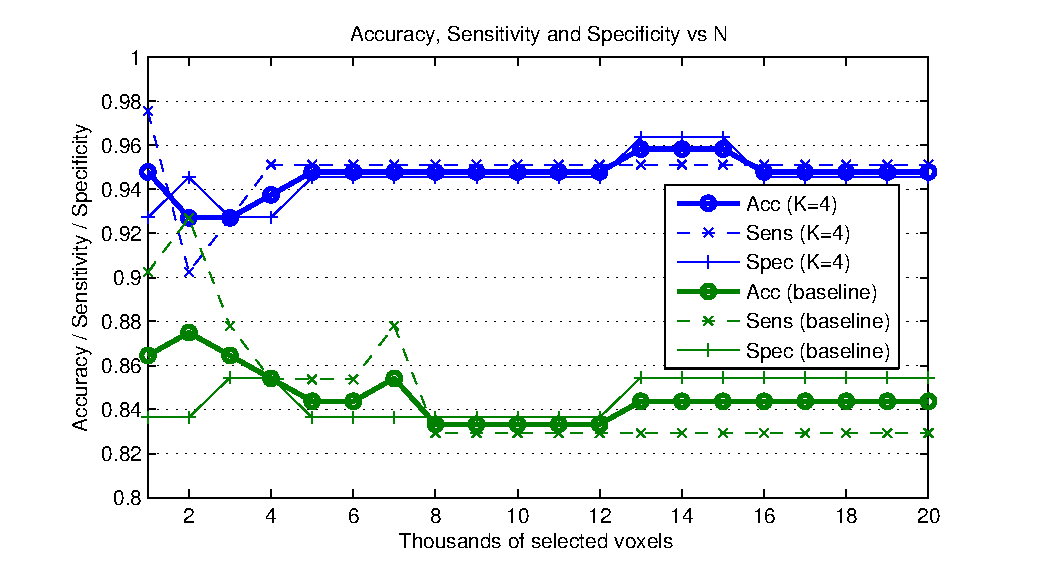
\includegraphics[width=.45\linewidth]{gfx/ch4/accsensspec_Vrel_vsN}} \quad
		\subfloat[Accuracy, Sensitivity and Specificity in function of $K$]
		{\label{fig:baseADvdln} %
			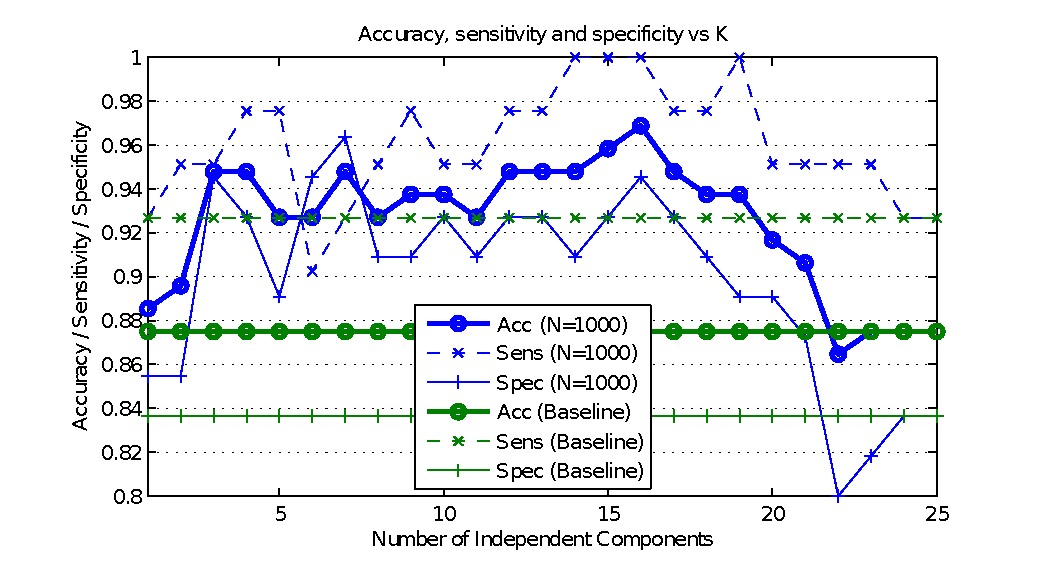
\includegraphics[width=.45\linewidth]{gfx/ch4/accsensspec_Vrel_vsK}}
		\caption{Accuracy, sensitivity and specificity values for a Quadratic Bayes classifier in function of the number of selected voxels and the number of features extracted, using the SPECT database. The highest value obtained by the baseline method is presented for comparison purposes in \ref{fig:baseADvdln}.}
		\label{fig:icaSPECTTodos}
	\end{figure*}
	
	
	Figure \ref{fig:icaSPECTTodos}(a) shows an interesting feature of this classifier. The final accuracy obtained is almost independent from the number of selected voxels. The obtained results are always better than the proposed baseline (SVAF) computed for the relative entropy criteria, and are always between $0.92$ and $0.97$. On the other hand, Figure Figure \ref{fig:icaSPECTTodos}(b) depicts the behaviour of the cited parameters when varying $K$. The values of accuracy, sensitivity and specificity ranges from $0.9$ to $0.97$ in a wide range (for $K$ between 3 and 20). The values obtained show the robustness of the proposed classifier for the SPECT database, and demonstrates its robustness in Alzheimer's Disease patterns detection as it provides high accuracy rates with a wide range operation.
	
	\subsubsection{ADNI-PET}
	For ADNI database, the behaviour is similar, but of lower values in evaluation parameters. Figure \ref{fig:icaADNITodos} depicts this behaviour, and compares it to the values obtained when evaluating the Relative Entropy baseline method. The proposed method shows values that are similar to those obtained with the baseline method, and shows, in general, an ascending trend by increasing the number of selected voxels.
	
	
	\begin{figure*}[bth]
		\myfloatalign
		\subfloat[Accuracy, Sensitivity and Specificity in function of $N$]
		{\label{fig:baseSPadni}%
			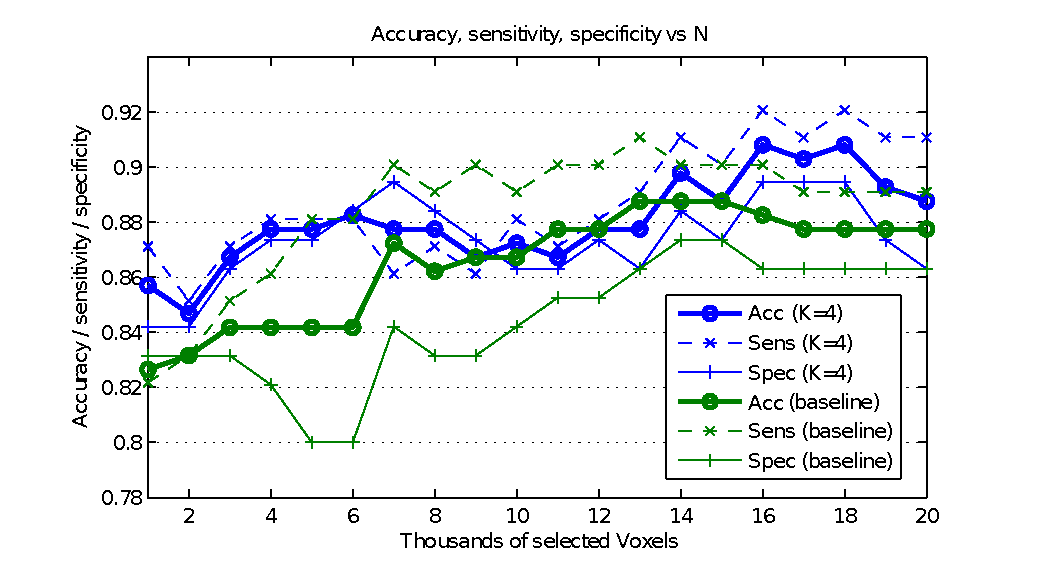
\includegraphics[width=.45\linewidth]{gfx/ch4/accsensspec_Arel_vsN}} \quad
		\subfloat[Accuracy, Sensitivity and Specificity in function of $K$]
		{\label{fig:baseADadni}%
			\includegraphics[width=.45\linewidth]{gfx/ch4/accsensspec_Arel_vsK}}
		\caption{Accuracy, sensitivity and specificity values for a SVM Linear classifier, in function of the number of selected voxels and the number of features extracted, using the ADNI database. The highest value obtained by the baseline method is presented for comparison purposes in \ref{fig:baseADadni}.}
		\label{fig:icaADNITodos}
	\end{figure*}
	
	
	As commented above, accuracy and sensitivity values trends to higher values when increasing the number of voxel selected $N$, as shown in Fig. \ref{fig:icaADNITodos}(a). Figure \ref{fig:icaADNITodos}(b) depicts these values in function of the number of features extracted $K$, and shows similar and occasionally lower values to those obtained for the baseline method. There are some increments on the evaluation parameters when using a $K$ value between 12 and 15, and $K=4$, as happened with the SPECT database. Despite this, the benefits of using a feature extraction with the ADNI database are not significant, or at least not in terms of these evaluation parameters. In terms of computational efficiency, the method proposed reduces the number of parameters used as input to the classifier, although it takes a longer time to estimate the independent components, which results also in small performance improvements over the baseline method.  
	
	\subsection{Parkinson's Disease}
	
	\subsubsection{Factor Analysis}
	
	\begin{figure*}
		\myfloatalign
		\subfloat[]{\includegraphics[width=0.5\textwidth]{gfx/ch4/accuracyMeanSTDFA_vsN_ttest}\label{fig:accFAvsNttest}}
		\subfloat[]{\includegraphics[width=0.5\textwidth]{gfx/ch4/accuracyMeanSTDFA_vsK_ttest}\label{fig:accFAvsKttest}}
		
		\caption{Accuracy values for the three \ac{PD}-related datasets: PPMI-DAT, VDLN-DAT and VDLV-DAT over \protect\subref{fig:accFAvsNttest} the number of voxels selected and \protect\subref{fig:accFAvsKttest} the number of components used.} 
		\label{fig:accFAttest}
	\end{figure*}
	
	\subsubsection{Independent Component Analysis}
	The second system tested is the one which combines selection of $N$ voxels, ranked by means of $t$-Test, Wilcoxon or Entropy criteria, the modeling of these feature vector using Independent Component Analysis (ICA) and a posterior classification step. Most representative results are shown on Table \ref{tab:detailedResults}.
	
	\begin{table*}[ht]
		\centering
		\begin{tabular}{lccccccc}
			Experiment 		& Method 	& Classifier	& Accuracy	& Sensitivity	& Specificity	& PL	& NL \\
			\hline \hline
			\multirow{3}{*}{\textbf{PPMI-Raw}} & Entropy & SVM-Lin & 0.903	& 0.982	& 0.851	& 6.61	& 0.021 \\ % (2,13,6)
			&	t-Test 	& SVM-Lin & 0.903	& 0.974	& 0.857	& 6.82	& 0.031 \\ % (5,10,6)
			&	Wilcoxon & SVM-Lin & 0.900	& 0.956	& 0.863	& 6.97	& 0.051 \\ % (6,10,6)
			\hline
			\multirow{3}{*}{\textbf{PPMI-1}} & Entropy 	& SVM-Lin	& 0.907	& 0.974	& 0.863	& 7.10	& 0.030 \\ % (21,16,6)
			& $t$-Test	& SVM-Lin	& 0.907	& 0.982	& 0.857	& 6.88	& 0.020 \\ % (10,16,6)
			& Wilcoxon	& SVM-Lin	& 0.913	& 0.991	& 0.863	& 7.23	& 0.010 \\ % (16,6,6)
			\hline
			\multirow{3}{*}{\textbf{PPMI-2}} & Entropy 	& SVM-Lin	& 0.900	& 0.965	& 0.857	& 6.75	& 0.041 \\ % (14,1,6)
			& $t$-Test	& SVM-RBF	& 0.896	& 0.956	& 0.857	& 6.69	& 0.051 \\ % (5,10,9)
			& Wilcoxon	& SVM-Lin	& 0.900	& 0.956	& 0.863	& 6.97	& 0.051 \\ % (6,10,6)
			\hline \hline
			\multirow{3}{*}{\textbf{VV-Raw}} & Entropy	& SVM-Lin & 0.928	& 0.935	& 0.920	& 11.69	& 0.070 \\ % (7,11,6)
			&	t-Test	& SVM-Lin 	& 0.923	& 0.917	& 0.930	& 13.10	& 0.090 \\ % (6,6,6)
			&	Wilcoxon & SVM-Lin & 0.923	& 0.926	& 0.920	& 11.57	& 0.081 \\ % (19,9,6)
			\hline
			\multirow{3}{*}{\textbf{VV-1}}	& Entropy	& SVM-Lin	& 0.928	& 0.935	& 0.920	& 11.69	& 0.070 \\ % (7,11,6)
			& $t$-Test	& SVM-Lin	& 0.923	& 0.917	& 0.930	& 13.10	& 0.090 \\ % (6,6,6)
			& Wilcoxon	& SVM-Lin	& 0.923	& 0.926	& 0.920	& 11.57	& 0.081 \\ %
			\hline
			\multirow{3}{*}{\textbf{VV-2}}	& Entropy	& SVM-RBF	& 0.938	& 0.954	& 0.920	& 11.92	& 0.050 \\ % (3,3,9)
			& $t$-Test	& SVM-RBF	& 0.947	& 0.981	& 0.910	& 10.91	& 0.020 \\ % (4,5,9)
			& Wilcoxon	& SVM-RBF	& 0.942	& 0.981	& 0.900	& 9.81	& 0.021 \\ % (4,6,9)
			
			\hline\hline
		\end{tabular}
		\caption{Best results of the complete system applied to the experiments proposed. Evaluation parameters of accuracy, sensitivity, specificity, PL and NL are shown. The classifier used to compute these results appears along with them and its corresponding experiment and selection criterion.}
		\label{tab:detailedResults}
	\end{table*}
	
	Table \ref{tab:detailedResults} shows the resulting evaluation parameters obtained with each experiment, database and selection criterion used. The classifier that perform better with each combination is also cited, which gives us an idea of the linearity of the distribution of the features in the ICA space. 
	
	The first interesting result that we infer from the table is that values obtained for the Experiment 1 and Raw are very similar in both databases, with similar values of accuracy, PL and NL, being the results obtained with Experiment 1 (with a mask) slightly higher than those obtained without the mask. This is very interesting, because it involves a relevant computational load reduction, which increases the performance of the live system, and also performs slightly better in some cases. On the other hand, the similarities between the results obtained with Experiment 1 and Raw show that the hypothesis testing methods used as selection criterion perform in a similar way to the mask. This suggests that both using a supervised method (a mask) or an unsupervised method (computed significance over the whole image) the results are almost the same, and then, our choice must be based on a trade-off between the computational load of the system and the addition (or not) of a supervised step. The difference of computational load varies between computing the significance maps for the whole brain, which contains $902629$ voxels in the PPMI database and $239805$ for the VV database, or the computation of those maps for the $1125$-$2606$ selected voxels of the striatum (depending on the database), which, as commented above, can be of great help in live systems. Both the usage of full images and the mask-based selection of voxels are equally valid, and both obtain similar results. 
	
	Regarding the Experiment 2, the obtained results behave in a different way depending on the database used. While the PPMI database obtains better results when there is no intensity normalization (in experiments PPMI-Raw and PPMI-1), the system obtains its highest performance when applied to a normalized VV database. 
	
	Before this behavior is analyzed, some details about the PPMI database must be pointed out. Due to the spatial normalization performed in the Raw PPMI images, some PD affected images show a deformation of the shape of the brain. This occurs because of the lower intensity of the striatum, due to lower amounts of dopamine in this area. When a template is used to register these images, the shape of the striatum differs substantially from that of the template (this is smaller, and of irregular shape), so that the resulting transformation could lead to a deformation of the striatum, and thus, of the whole brain, in order to match the template. Thereby some brain coordinates do not match the same anatomical position, which can lead to a misclassification.
	
	Also, in PPMI database, an attenuation correction using a cobalt line marker (as commented in Section \ref{sec:ppmi}) has been performed. This line marker facilitates the image processing and distinguishes left and right sides for manual processing. However, this adds a non-relevant area in the images with values similar to those of the striatum, which experiments Raw and 2 can take into account, unlike experiment 1 that uses a mask to select the ROI. This combination of high-intensity non-relevant areas, brain deformations due to low intensity striatum and attenuation correction of the images could cause the lower performance values obtained in the Experiment 2 when applied to PPMI database. 
	
	On the other hand, best performance results are obtained when using an intensity normalization step in the VV database. As only spatially-normalized images are used, the intensity normalization procedure features an increment in the accuracy, and a significant decrement in the NL values. Compared to Experiment 1, where only a mask is applied to the images, values obtained using either $t$-Test or MWW perform significantly better. Due to the aforementioned intensity normalization, values of the striatum in the Experiment 2 are comparable, while those of the Experiment 1 are not. However, the Raw images should present differences, since high accuracy values are also obtained with Experiments VV-Raw and VV-1. 
	
	The last comment of this table concerns the classifiers that better match each experiment and voxel selection criterion. The best classifier is very representative of the spatial distribution that the projected features present on the ICA space. Linear classifiers such as SVM usually fit linearly separable classes, which can result in a good projection of the features into the ICA space. But SVM Linear performs as the best classifier when using random distributed classes too. On the contrary, non-linear classifiers such as the SVM-RBF, reveal classes that are non-linearly separable, and therefore, achieve best performance because they conform to best shape the spatial distribution of ICA projections in space. While using SVM-Lin or RBF in experiments Raw and 1 do not vary the performance of the system (e.g, using SVM-RBF in PPMI-Raw leads to accuracy results around $0.90$ and using it with VV-1 achieves an accuracy around $0.93$), the intensity normalization procedure seems to vary the spatial distribution of the independent components, specially with the VV database, making a non-linear kernel (RBF) to better fit those and obtain better results. 
	
	Because the differences between Experiment Raw and 1 have not been significant beyond the computational load, we will concentrate on the difference of the performance in using intensity-normalized images or not. As the PPMI database was attenuation corrected and, regarding the results obtained for Experiments Raw and 2, this can be considered as an intensity normalization procedure, we will concentrate on the results obtained for PPMI-Raw. In the case of VV database, we will analyze both the results obtained for experiment Raw (unnormalized) and 2 (normalized), and compare the performance obtained in both experiments
	
	To better illustrate the variations of the performance values along the different variables $N$ (number of selected voxels) and $K$ (number of independent components used), the accuracy obtained for each of the experiments proposed above (PPMI-Raw, VV-Raw and VV-2) when varying the input parameters of the system are shown on Figure \ref{fig:accExperimentsWithouthMask}.
	
	\begin{figure*}
		\centering
		\subfloat[]{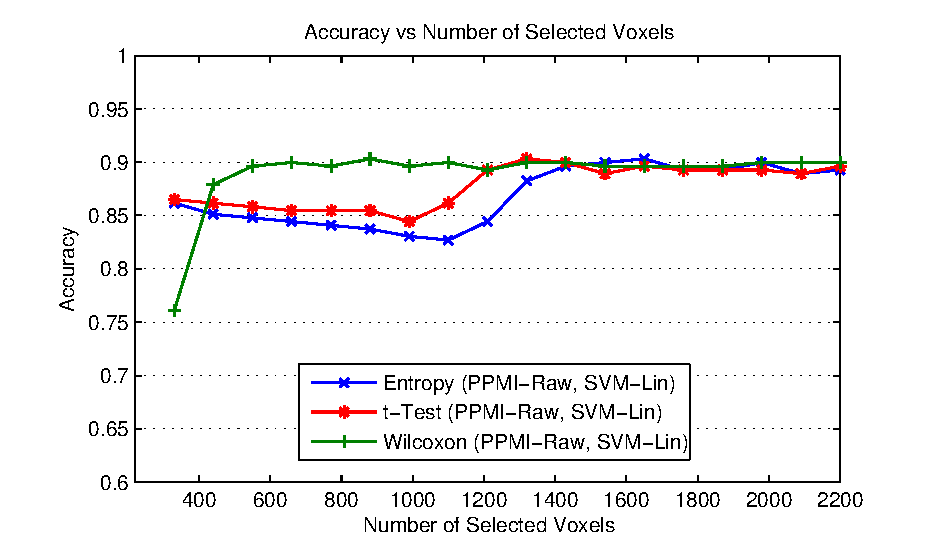
\includegraphics[width=0.49\textwidth]{gfx/ch4/AccuracyPPMI2.eps}\label{fig:PPMI1vsNacc}}
		\subfloat[]{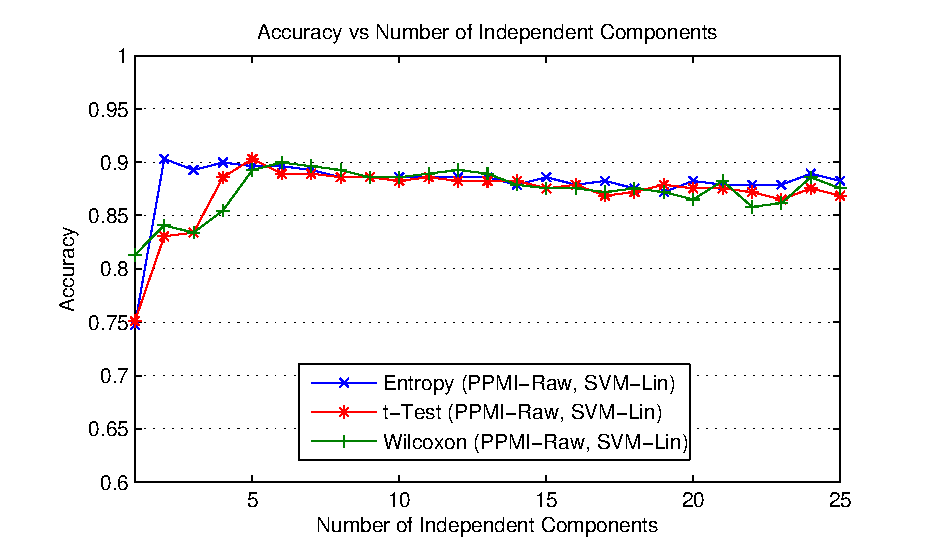
\includegraphics[width=0.49\textwidth]{gfx/ch4/accuracyPPMI2vsK.eps}\label{fig:PPMI1vsKacc}}
		
		\subfloat[]{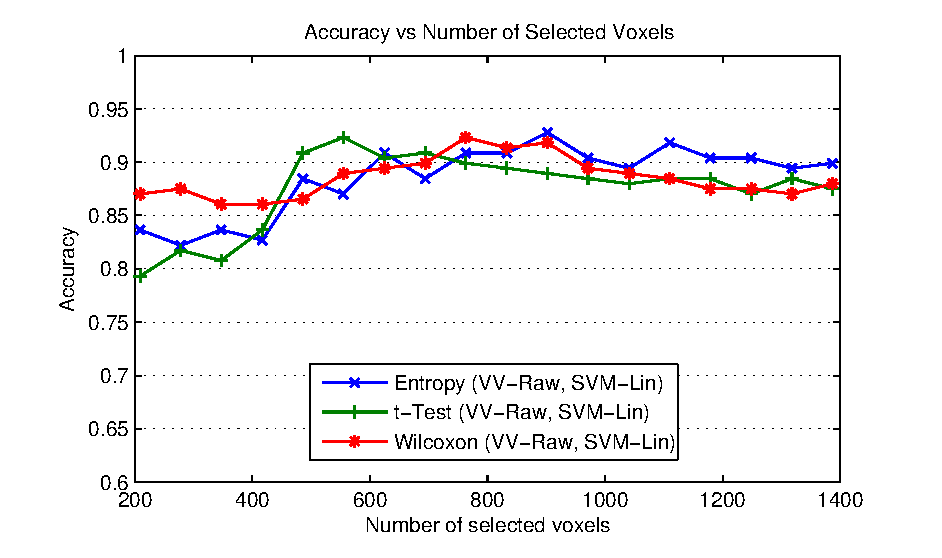
\includegraphics[width=0.49\textwidth]{gfx/ch4/accuracyVVRawvsN.eps}\label{fig:VVRawvsNacc}}
		\subfloat[]{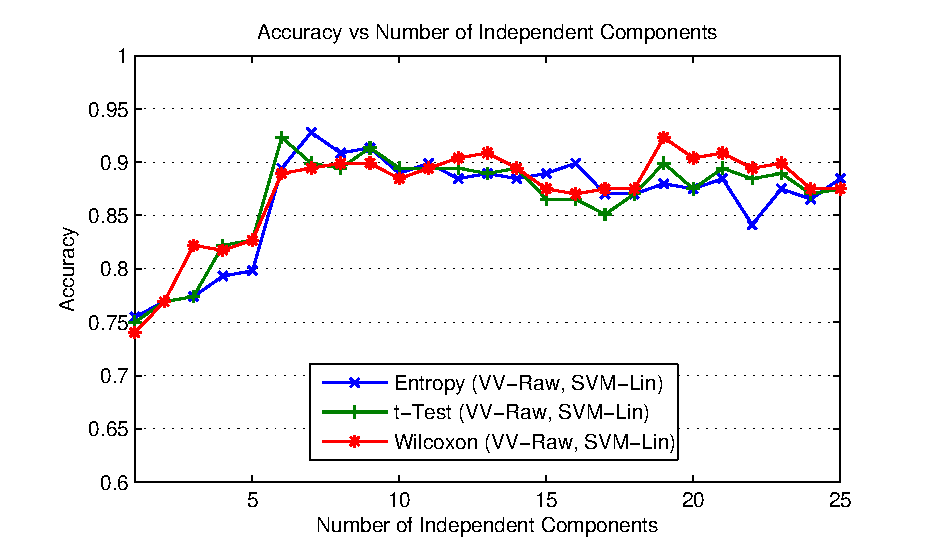
\includegraphics[width=0.49\textwidth]{gfx/ch4/accuracyVVRawvsK.eps}\label{fig:VVRawvsKacc}}
		
		\subfloat[]{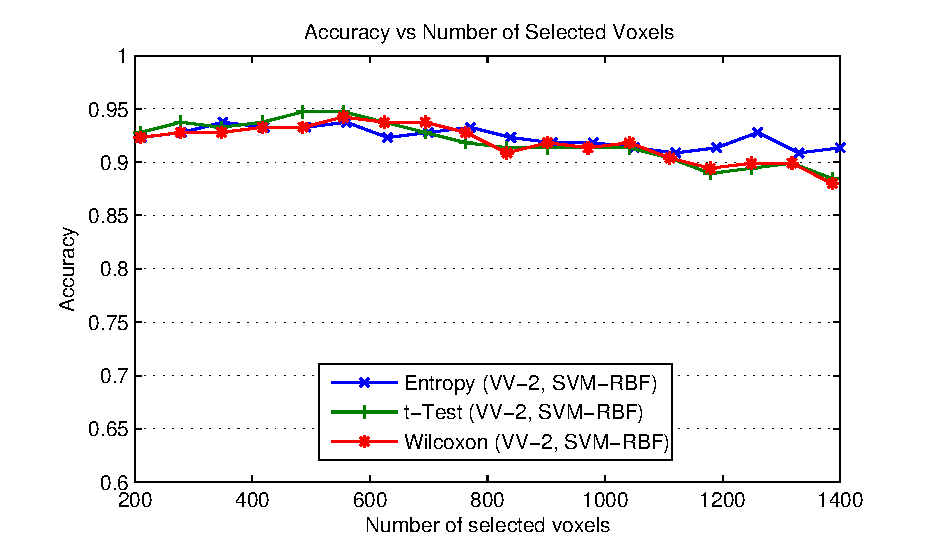
\includegraphics[width=0.49\textwidth]{gfx/ch4/accuracyVV2vsN.eps}\label{fig:VV2vsNacc}}
		\subfloat[]{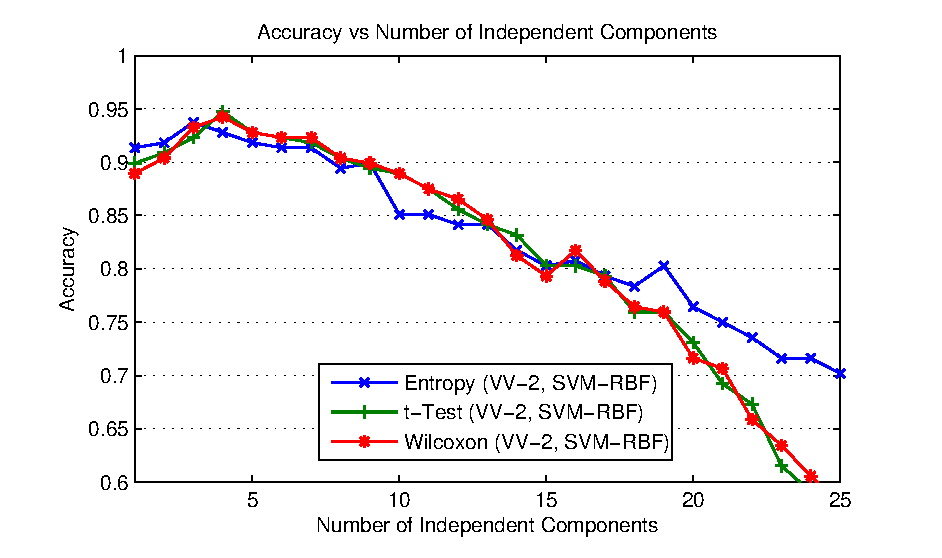
\includegraphics[width=0.49\textwidth]{gfx/ch4/accuracyVV2vsK.eps}\label{fig:VV2vsKacc}}
		
		\caption{Accuracy values over $K$ and $N$ for: \ref{fig:PPMI1vsNacc} and \ref{fig:PPMI1vsKacc}) experiment PPMI-Raw; \ref{fig:VVRawvsNacc} and \ref{fig:VVRawvsKacc}) experiment VV-Raw; and \ref{fig:VV2vsNacc} and \ref{fig:VV2vsKacc}) experiment VV-2.} 
		\label{fig:accExperimentsWithouthMask}
	\end{figure*}
	
	Fig. \ref{fig:PPMI1vsNacc} and \ref{fig:PPMI1vsKacc} show the accuracy values obtained for experiment PPMI-Raw and each of the selection criteria. Those images feature, as commented, an attenuation correction that performs similarly to an intensity normalization procedure, leading to similar results in the three experiments proposed (Raw, 1 and 2). The number of selected voxels that we have evaluated is higher than that used for VV database, due to the higher size of images in the PPMI database. The accuracy plots shows that performance values remain almost constant in values around $0.9$ for every experiment and selection criterion (in selected operation ranges). Particularly, when regarding the $N$ values in Fig. \ref{fig:PPMI1vsNacc}, there is an interesting behavior in the graphs showing how different selection methods lead to different operation ranges. A sort of voxel threshold divides the accuracy in two values: around $0.85$ and $0.9$, and this threshold varies between $400$ voxels for MWW selection criterion and $1400$ voxels for Relative Entropy. Therefore, the method that better measures the significance of voxels is the one that achieves better values of accuracy with a smaller number of voxels. 
	
	However, the behavior in Fig. \ref{fig:PPMI1vsKacc}, that depicts how the performance values vary with a different number of independent components ($K$) offer different results. In fact, best values are obtained with lower $K$, especially when using a Relative Entropy selection criterion. This means that the independent components are better modeled when it takes into account the voxels selected using relative entropy significance measures. On the other hand, either $t$-Test and MWW offer similar results, as expected. But the point here is the high accuracy values around $0.9$ and with low variation along the number of components extracted. 
	
	In \ref{fig:VVRawvsNacc} and \ref{fig:VVRawvsKacc}, accuracy results for the VV-Raw experiment are shown. The images used on VV-Raw were only spatially-normalized, so no comparisons can be made between intensity levels a priori. However, the relationships between striatum values and the remaining areas of the brain are very similar among Parkinson-affected  images, and so it happens in normal control images.  As significance values have been obtained using three different hypothesis testing methods among all images, and these significance measures are computed according to intensity values -which are not comparable a priori-, it is possible to think that there will be a number of noisy voxels which will reduce the performance of the classifier. That explains the variations of the accuracy on Figures \ref{fig:VVRawvsNacc} and \ref{fig:VVRawvsKacc}. In Fig. \ref{fig:VVRawvsNacc} low accuracy values are obtained with a lower number of voxels, but the performance increases as a higher number of voxels are considered. Due to the aforementioned reasons, it is also reasonable to assume that the estimation of the independent components will be better as the number of selected voxels increases, and so will the performance of the classifier.
	
	Regarding the accuracy variations in function of $K$, it is also interesting to note that we need a high number of components (more than $6$) to achieve good accuracy results. This is probably due to the intensity differences between different images of the same class, and between images of different classes. As has been commented before, we needed a higher number of voxels to obtain good performance results, and probably some of those were non-relevant noisy voxels that obtained higher significance values due to the lack of intensity normalization. Therefore, a higher number of independent components are needed to better model these vectors that contain both significant and noisy voxels. Finally, to focus on the operating ranges, for experiment VV-Raw we obtain good results of accuracy in a range of $N > 600$ and $K>6$, although it might slightly vary depending on the selection criterion used.
	
	Fig. \ref{fig:VV2vsNacc} and \ref{fig:VV2vsKacc} depict accuracy values for experiment VV-2. Here, it is important to highlight the high values and robustness of the accuracy values over $N$, which are obtained using either of the significance computation methods proposed. Due to the intensity normalization applied to the images of the database, the system outperforms the VV-Raw, obtaining a robust performance and almost totally avoiding dependence on the number of voxels selected $N$. Accuracy values over $K$ perform slightly different to the previous two experiments, mainly due to the different classifier used here. Best values are obtained in the first $5$ independent components, and from this point on, the performance of the system degrades, which is a typical behavior of using non-linear kernels. A number of components of $K=4,5$ is optimum for this application. This is probably due to the peaking phenomenon \cite{Krishnaiah1982}. The peaking phenomenon describes how the use of complex classifiers leads to a better fitting of the training data, but degrading its generalization properties. Then, an increment in the size of the training data (a new IC added) leads to an increment in the complexity of the classifier, at the expense of the generalization ability of the classifier. Therefore, as the number of IC increases, the generalization capabilities of the classifier decrease, and so does the performance of the system. Since this problem is exacerbated by the complexity of the system, this will occur much faster with an RBF kernel than with a Linear one.
	
	
	
	\begin{table*}[ht]
		\centering
		\begin{tabular}{lcccccccc}
			Experiment 		& Kernel & Over & Method 	& Accuracy	& Sensitivity	& Specificity	& PL	& NL \\
			\hline \hline
			\multirow{12}{*}{\textbf{PPMI-Raw}} & \multirow{6}{*}{\textbf{Linear}} & \multirow{3}{*}{N}	& Entropy	& 0.887	& 0.954	& 0.843	& 6.10	& 0.055 \\ % (5)
			&	&	& $t$-Test	& 0.881	& 0.945	& 0.839	& 5.87	& 0.065 \\ % (13)
			&	&	& Wilcoxon	& 0.881	& 0.950	& 0.835	& 5.78	& 0.060 \\ % (18)
			\cline{3-9}
			& & \multirow{3}{*}{K}	& Entropy	& 0.888	& 0.962	& 0.841	& 6.05	& 0.046 \\ % (6)
			&	&	& $t$-Test	& 0.881	& 0.950	& 0.835	& 5.78	& 0.060 \\ % (18)
			&	&	& Wilcoxon	& 0.882	& 0.942	& 0.842	& 5.97	& 0.070 \\ % (10)
			\cline{2-9}
			& \multirow{6}{*}{RBF} & \multirow{3}{*}{N}	& Entropy	& 0.874	& 0.942	& 0.830	& 5.60	& 0.070 \\ % (5)
			&	&	& $t$-Test	& 0.873	& 0.933	& 0.834	& 5.70	& 0.080 \\ % (5)
			&	&	& Wilcoxon	& 0.895	& 0.960	& 0.853	& 6.53	& 0.047 \\ % (5)
			\cline{3-9}
			& & \multirow{3}{*}{K}	& Entropy	& 0.873	& 0.918	& 0.844	& 5.93	& 0.097 \\ % (13)
			&	&	& $t$-Test	& 0.867	& 0.917	& 0.834	& 5.72	& 0.099 \\ % (14)
			&	&	& Wilcoxon	& 0.878	& 0.916	& 0.854	& 6.26	& 0.099 \\ % (5)
			\hline
			\multirow{12}{*}{\textbf{VV-2}} & \multirow{6}{*}{Linear} & \multirow{3}{*}{N}	& Entropy	& 0.911	& 0.923	& 0.899	& 9.16	& 0.086 \\ % (4)
			&	&	& $t$-Test	& 0.917	& 0.937	& 0.895	& 9.00	& 0.070 \\ % (10)
			&	&	& Wilcoxon	& 0.917	& 0.940	& 0.894	& 8.86	& 0.068 \\ % (11)
			\cline{3-9}
			& & \multirow{3}{*}{K}	& Entropy	& 0.899	& 0.914	& 0.883	& 7.93	& 0.098 \\ % (18)
			&	&	& $t$-Test	& 0.902	& 0.918	& 0.885	& 8.06	& 0.093 \\ % (14)
			&	&	& Wilcoxon	& 0.902	& 0.916	& 0.888	& 8.25	& 0.095 \\ % (14)
			\cline{2-9}
			& \multirow{6}{*}{\textbf{RBF}}	& \multirow{3}{*}{N}	& Entropy	& 0.929	& 0.959	& 0.897	& 9.39	& 0.045 \\ % (4)
			&	&	& $t$-Test	& 0.926	& 0.965	& 0.885	& 8.48	& 0.040 \\ % (5)
			&	&	& Wilcoxon	& 0.926	& 0.966	& 0.884	& 8.39	& 0.039 \\ % (5)
			\cline{3-9}
			& & \multirow{3}{*}{K}	& Entropy	& 0.915	& 0.958	& 0.869	& 7.92	& 0.048 \\ % (3)
			&	&	& $t$-Test	& 0.919	& 0.957	& 0.878	& 8.44	& 0.049 \\ % (1)
			&	&	& Wilcoxon	& 0.917	& 0.952	& 0.880	& 8.42	& 0.054 \\ % (1)
			
			\hline\hline
		\end{tabular}
		\caption{Average accuracy, sensitivity, specificity, and PL and NL computed for each significance estimation method, over two parameters: $N$ and $K$, regarding the two kernel methods.  }
		\label{tab:meanValuesPPMIVV}
	\end{table*}
	
	As seen in these figures, the method used to estimate voxel significance has no relevant impact on later outcomes. To illustrate better this result, Table \ref{tab:meanValuesPPMIVV} summarizes the average parameters for the PPMI-Raw and VV-2 experiments. As we have tested the benefits of using the intensity normalization algorithm in the database, experiment VV-Raw will be obviated from this moment. These average values are computed over $N$ and over all $K$ for PPMI-Raw and the first $10$ independent components for VV-2 for each significance estimation method, using either Linear or RBF kernel in both databases, to better illustrate the behavior of the system. 
	
	These average accuracy values range between $0.88$ and $0.89$ for PPMI-Raw and over $0.92$ when computed over $N$ for experiment VV-2 (SVM-RBF). Average values computed over $K$ for experiment VV-2 are not very relevant because, as commented before, the performance of the classifier decreases when the number of components increases due to the peaking phenomenon. A slightly decrease on the performance of the system when we use the Linear kernel is noticeable in this case, although maintaining good performance values. Both systems hold small dependence of the number of voxels $N$ and, when a linear classifier is used, of the number of components $K$. Positive and Negative Likelihood values obtained are lower in PPMI database than in VV database. As commented in Section \ref{sec:results} values of PL over 8 are very likely for the patient to suffer from a specific diagnosis, so values obtained for VV-2 experiment are very representative. 
	
	Regarding the PPMI database, although accuracy, sensitivity specificity, PL and NL values are good, and the classifier shows its robustness against variation in the input parameters $K$ and $N$, the performance showed by this system does not equal that obtained by the VV-2 experiment. This can be due to both the aforementioned attenuation correction and the spatial normalization difficulties. Using a RBF kernel here provides no improvements, and also decreases the performance values in most cases. The best average values for PPMI database are obtained when considering a system composed by Relative Entropy significance measure, ICA for feature extraction when using SVM-Lin and the Mann-Whitney-Wilcoxon $U$-test when using SVM-RBF. For VV database, similar average values are obtained by any of the selection criteria and using SVM-RBF. We finally choose Relative Entropy criterion by analogy with the experiment PPMI-Raw. Average values of accuracy, sensitivity and specificity for each of these systems (Relative Entropy + ICA + SVM Classifier), computed along $N$ and $K$ are shown in Figure \ref{fig:meanParameters}.
	
	
	\begin{figure*}
		\centering
		\subfloat[]{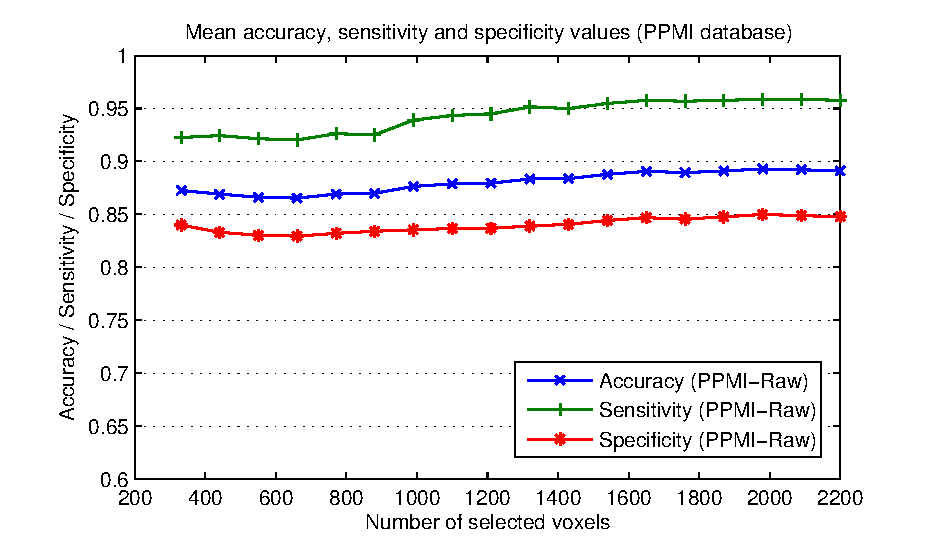
\includegraphics[width=0.49\textwidth]{gfx/ch4/meanParametersPPMIvsN.eps}\label{fig:PPMImeanvsN}}
		\subfloat[]{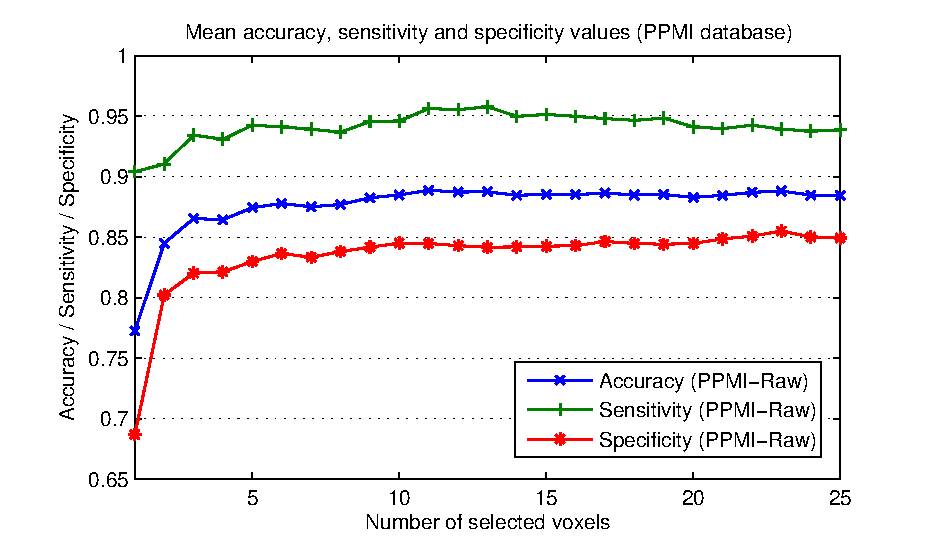
\includegraphics[width=0.49\textwidth]{gfx/ch4/meanParametersPPMIvsK.eps}\label{fig:PPMImeanvsK}}
		
		\subfloat[]{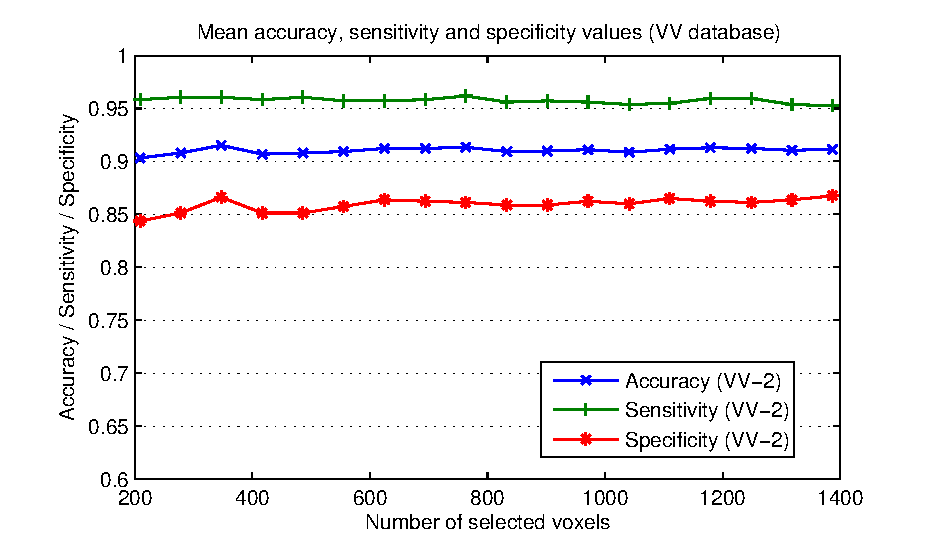
\includegraphics[width=0.49\textwidth]{gfx/ch4/meanParametersVVvsN.eps}\label{fig:VVmeanvsN}}
		\subfloat[]{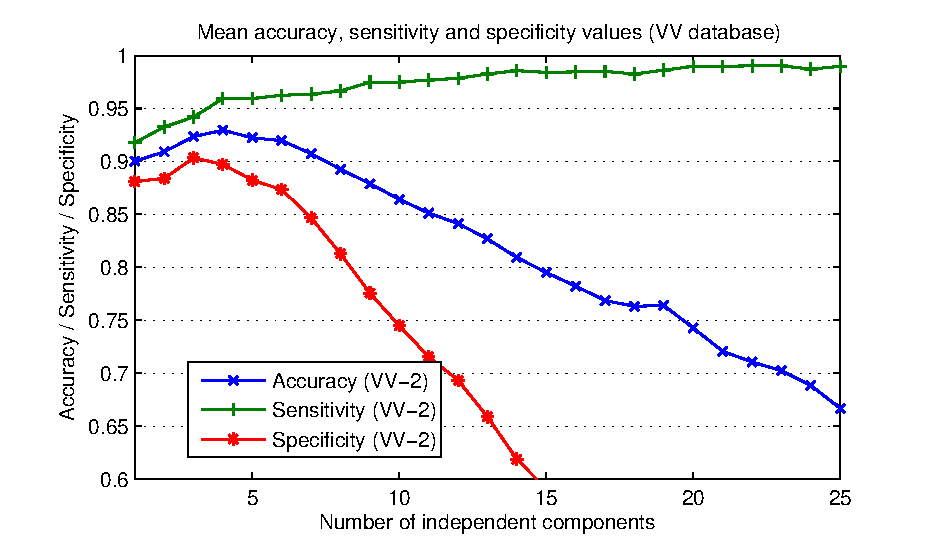
\includegraphics[width=0.49\textwidth]{gfx/ch4/meanParametersVVvsK.eps}\label{fig:VVmeanvsK}}
		
		\caption{Average values of the evaluation parameters: accuracy, sensitivity and specificity, for a system composed of a relative entropy selection criterion and a SVM classifier. Values obtained for experiments PPMI-Raw and VV-2.} 
		\label{fig:meanParameters}
	\end{figure*}
	%hasta aquí. 
	
	Finally, we look at the ROC curves obtained by the proposed system in \ref{fig:rocPPMI}) PPMI database and \ref{fig:rocVV}) VV database. The performance of the system by means of its sensitivity-specificity trade-off is displayed using the three alternative significance estimation methods proposed previously, along with the performance obtained by the VAF approach, using the provided images in the case of PPMI and the intensity-normalized images in the case of VV.  It is interesting to note that, as we have commented above, the performance obtained by the three significance estimation methods is very similar, with similar operation points, although the differences among them are bigger in the PPMI database. The systems proposed perform in both cases better than the VAF-based systems, which is widely considered as an estimation of the performance of a visual analysis performed by expert clinicians \cite{Stoeckel04}.
	
	\begin{figure*}
		\centering
		\subfloat[]{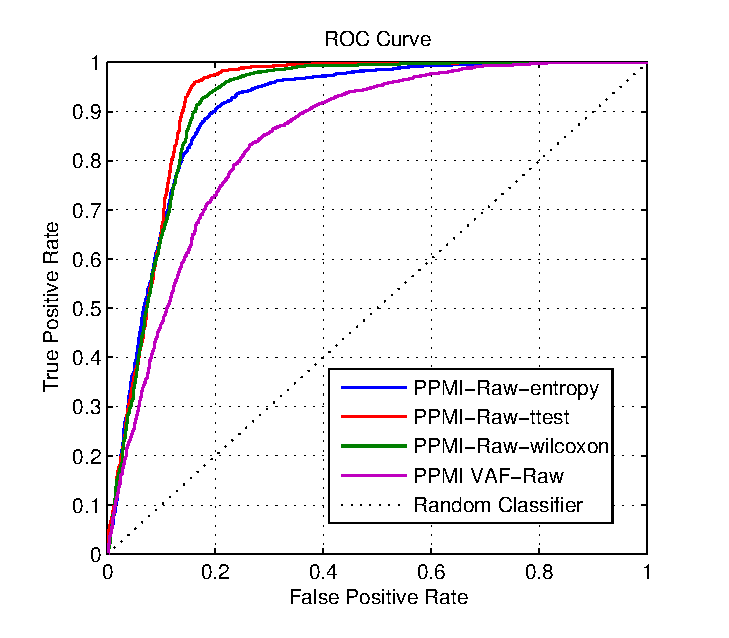
\includegraphics[width=0.4\textwidth]{gfx/ch4/ROC_PPMI_nuevo.eps}\label{fig:rocPPMI}}
		\subfloat[]{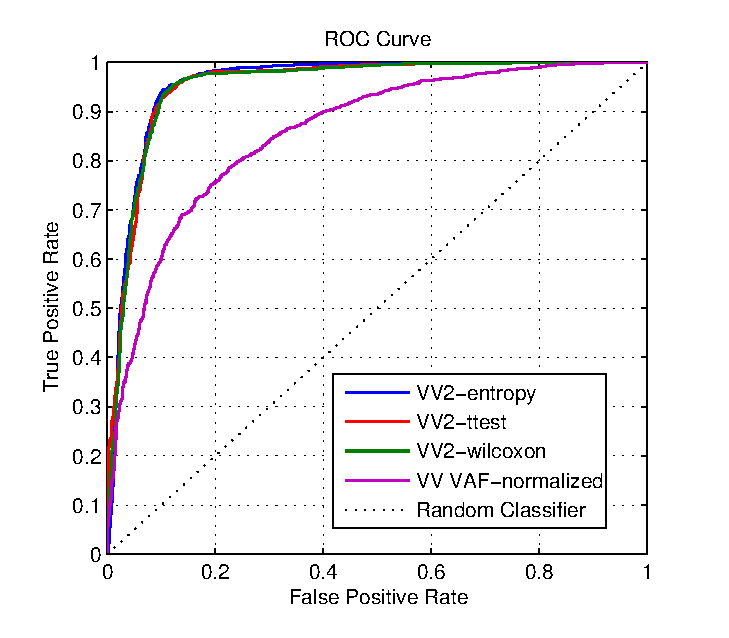
\includegraphics[width=0.4\textwidth]{gfx/ch4/ROC_VV_nuevo.eps}\label{fig:rocVV}}
		
		\caption{ROC curves obtained with the systems proposed in experiments PPMI-Raw and VV-2 for (a) PPMI database and (b) VV database, and compared to their respective VAF systems. } 
		\label{fig:roccurve}
	\end{figure*}
